Der Effekt einer Chirurgie auf die niederen Homologiegruppen ist recht simpel. Sei \(n=i+j+1\), \(\mathcal{M}^n\) eine Mannigfaltigkeit, \(\mathcal{S}^i\hookrightarrow\mathcal{M}\) eine eingebettete Sph\"are mit trivialem Normalenb\"undel und \(\Phi\colon\underline{\mathbb{D}}^{j+1}\hookrightarrow\mathcal{M}\) eine zugeh\"orige Anklebeeinbettung. Setze \(\mathcal{D}:=\im\Phi\) und
\[\mathcal{M}_0:=\mathcal{M}\setminus\mathring{\mathcal{D}}\quad\text{sowie}\quad\mathcal{M}^{\prime}:=\mathcal{M}_0\cup_{\partial\mathcal{D}}\left(\mathbb{D}^{i+1}\times\mathbb{S}^j\right)\,.\] 
Dann lassen sich die langen exakten Folgen der Paare \((\mathcal{M},\mathcal{M}_0)\) und \((\mathcal{M}^{\prime},\mathcal{M}_0)\) zu folgendem Diagramm zusammensetzen:
\begin{center}
    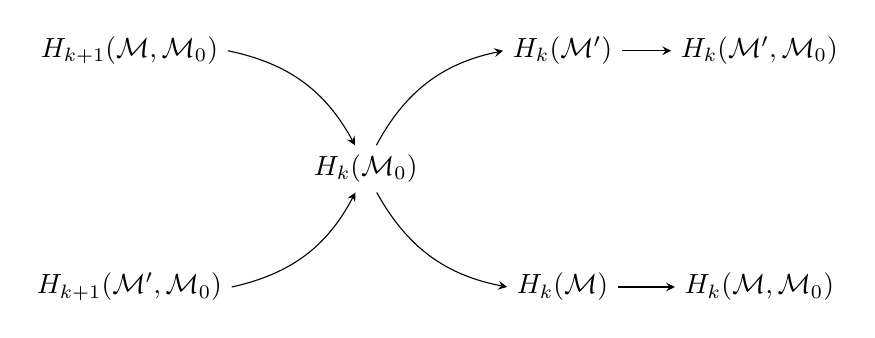
\begin{tikzpicture}
        \draw
            (-3, -1.5) node (B) {\(H_{k+1}(\mathcal{M}^{\prime},\mathcal{M}_0)\)}
            (0, 0) node (C) {\(H_k(\mathcal{M}_0)\)}
            (2.5, 1.5) node (D) {\(H_k(\mathcal{M}^{\prime})\)}
            (5, 1.5) node (E) {\(H_k(\mathcal{M}^{\prime},\mathcal{M}_0)\)}
            (-3, 1.5) node (G) {\(H_{k+1}(\mathcal{M},\mathcal{M}_0)\)}
            (2.5, -1.5) node (H) {\(H_k(\mathcal{M})\)}
            (5, -1.5) node (I) {\(H_k(\mathcal{M},\mathcal{M}_0)\)}
            
            (B.east) edge [bend right = 25, -stealth] (C)
            (C) edge [bend left = 25, -stealth] (D.west)
            (D) edge [-stealth] (E)

            (G.east) edge [bend left = 25, -stealth] (C)
            (C) edge [bend right = 25, -stealth] (H.west)
            (H) edge [-stealth] (I)
            ;
    \end{tikzpicture}
\end{center}
Per Ausschneidung folgen
\[H_k(\mathcal{M},\mathcal{M}_0)\cong H_k(\mathbb{S}^i\times\mathbb{D}^{j+1},\mathbb{S}^i\times\mathbb{S}^j)\cong\begin{cases}
    \mathbb{Z} & k\in\{0,j+1\}\\
    0 & 0<k<j+1
\end{cases}\]
und 
\[H_k(\mathcal{M}^{\prime},\mathcal{M}_0)\cong H_k(\mathbb{D}^{i+1}\times\mathbb{S}^j,\mathbb{S}^i\times\mathbb{S}^j)\cong\begin{cases}
    \mathbb{Z} & k\in\{0,i+1\}\\
    0 & 0<k<i+1
\end{cases}\,.\]
F\"ur die Berechnung siehe Appendix. Die Erzeuger der \(\mathbb{Z}\)-Anteile in Dimension \(i+1\) und \(j+1\) sind gerade die Bilder der Erzeuger von \(H_{i+1}(\mathbb{D}^{i+1},\mathbb{S}^i)\) und \(H_{j+1}(\mathbb{D}^{j+1},\mathbb{S}^j)\) und stehen somit in Korrespondenz zu Fundamentalklassen eines \"Aquators \(e=\Phi(x\times\mathbb{S}^j)\) und einem Meridian \(m=\Phi(\mathbb{S}^i\times y)\). \"Aquator und Meridian sind deswegen interessant, da sie beide in \(\mathcal{M}_0\) liegen, und die Beziehungen
\[\eqcl{e\mathrel{|}\mathcal{M}}=\eqcl{\mathcal{S}\mathrel{|}\mathcal{M}},\quad\eqcl{m\mathrel{|}\mathcal{M}}=0\quad\text{sowie}\quad\eqcl{e\mathrel{|}\mathcal{M}^{\prime}}=0\]
erf\"ullen. Die Sph\"are hei\ss e \textbf{primitiv}, wenn ein \(g\in H_j(\mathcal{M})\) mit \(g\cdot\eqcl{\mathcal{S}\mathrel{|}\mathcal{M}}=1\) existiert.
\begin{lemma}
    Chirurgie an einer Sph\"are \(\mathcal{S}^i\hookrightarrow\mathcal{M}^n\) mit \(i<j\) eliminiert die Fundamentalklasse \(\eqcl{\mathcal{S}\mathrel{|}\mathcal{M}}\).
\end{lemma}
\begin{proof}
    Einerseits folgt f\"ur \(1<k<i\) direkt
    \[H_k(\mathcal{M}^{\prime})\cong H_k(\mathcal{M}_0)\cong H_k(\mathcal{M})\,.\]
    Das Diagramm nimmt f\"ur \(k=i\) die folgende Form an:
    \begin{center}
        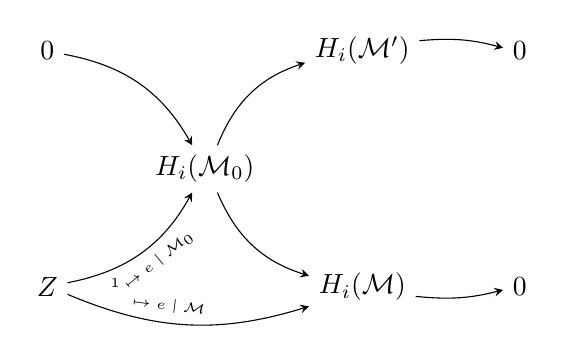
\begin{tikzpicture}
            \draw
                (-2, -1.5) node (B) {\(\mathbb{Z}\)}
                (0, 0) node (C) {\(H_i(\mathcal{M}_0)\)}
                (2, 1.5) node (D) {\(H_i(\mathcal{M}^{\prime})\)}
                (4, 1.5) node (E) {\(0\)}
                (4, -1.5) node (F) {\(0\)}
                (-2, 1.5) node (G) {\(0\)}
                (2, -1.5) node (H) {\(H_i(\mathcal{M})\)}

                (B) edge [bend right = 25, -stealth] node [below = 0.17, pos = 0.3] {\tiny\(1\)} node [sloped, below, pos = 0.56] {\tiny\(\mapsto\eqcl{e\mathrel{|}\mathcal{M}_0}\)} (C)
                (C) edge [bend left = 25, -stealth] (D)
                (D) edge [bend left = 10, -stealth] (E)

                (B) edge [bend right = 20, -stealth] node [sloped, above, pos = 0.41] {\tiny\(\mapsto\eqcl{e\mathrel{|}\mathcal{M}}\)} (H)

                (G) edge [bend left = 25, -stealth] (C)
                (C) edge [bend right = 25, -stealth] (H)
                (H) edge [bend right = 10, -stealth] (F)
                ;
        \end{tikzpicture}
    \end{center}
    Somit gilt 
    \[H_i(\mathcal{M}^{\prime})\cong H_i(\mathcal{M}_0)/\langle\eqcl{e\mathrel{|}\mathcal{M}_0}\rangle\cong H_i(\mathcal{M})/\langle\eqcl{e\mathrel{|}\mathcal{M}}\rangle\,.\]
\end{proof}
Auf \"ahnliche Art und Weise kann der Effekt einer Chirurgie auf die Homotopiegruppen untersucht werden.
\begin{lemma}\label{lem:fund_smaller}
    F\"ur \(k<i<j\) existiert ein Normalteiler \(N\triangleleft\pi_i(\mathcal{M})\) mit \(\eqcl{\mathcal{S}}\in N\) und
    \[\pi_k(\mathcal{M}^{\prime})\cong\pi_k(\mathcal{M})\quad\text{und}\quad\pi_i\left(\mathcal{M}^{\prime}\right)\cong\pi_i(\mathcal{M})/N\,.\]
\end{lemma}
\begin{lemma}\label{lem:odd_surg_effect}
    Chirurgie an einer \textbf{primitiven} Sph\"are \(\mathcal{S}^i\hookrightarrow\mathcal{M}^{2i+1}\) eliminiert die Fundamentalklasse \(\eqcl{\mathcal{S}\mathrel{|}\mathcal{M}}\).
\end{lemma}
\begin{proof}
    Es gilt \(i=j\). Das Diagramm nimmt die folgende Form an:
    \begin{center}
        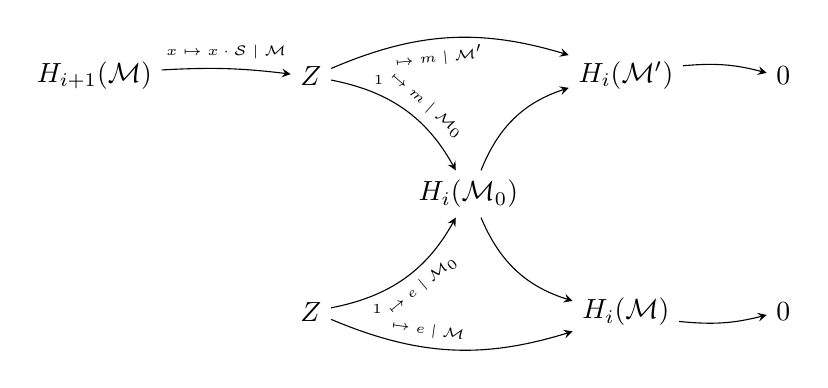
\begin{tikzpicture}
            \draw
                (-4.75, 1.5) node (A) {\(H_{i+1}(\mathcal{M})\)}
                (-2, -1.5) node (B) {\(\mathbb{Z}\)}
                (0, 0) node (C) {\(H_i(\mathcal{M}_0)\)}
                (2, 1.5) node (D) {\(H_i(\mathcal{M}^{\prime})\)}
                (4, 1.5) node (E) {\(0\)}
                (4, -1.5) node (F) {\(0\)}
                (-2, 1.5) node (G) {\(\mathbb{Z}\)}
                (2, -1.5) node (H) {\(H_i(\mathcal{M})\)}

                (A) edge [-stealth, bend left = 5] node [above] {\tiny\(x\mapsto x\cdot\eqcl{\mathcal{S}\mathrel{|}\mathcal{M}}\)} (G)
                (B) edge [bend right = 25, -stealth] node [below = 0.17, pos = 0.29] {\tiny\(1\)} node [sloped, below, pos = 0.56] {\tiny\(\mapsto\eqcl{e\mathrel{|}\mathcal{M}_0}\)} (C)
                (C) edge [bend left = 25, -stealth] (D)
                (D) edge [bend left = 10, -stealth] (E)

                (B) edge [bend right = 20, -stealth] node [sloped, above, pos = 0.39] {\tiny\(\mapsto\eqcl{e\mathrel{|}\mathcal{M}}\)} (H)
                (G) edge [bend left = 20, -stealth] node [sloped, below, pos = 0.45] {\tiny\(\mapsto\eqcl{m\mathrel{|}\mathcal{M}^{\prime}}\)} (D)

                (G) edge [bend left = 25, -stealth] node [above = 0.19, pos = 0.3] {\tiny\(1\)} node [sloped, above, pos = 0.59] {\tiny\(\mapsto\eqcl{m\mathrel{|}\mathcal{M}_0}\)} (C)
                (C) edge [bend right = 25, -stealth] (H)
                (H) edge [bend right = 10, -stealth] (F)
                ;
        \end{tikzpicture}
    \end{center}
    Da die Sph\"are primitiv ist, ist \(H_{i+1}(\mathcal{M})\to\mathbb{Z}\) surjektiv, also \(H_i(\mathcal{M})\cong H_i(\mathcal{M}_0)\). Es folgt 
    \[H_i(\mathcal{M}^{\prime})\cong H_i(\mathcal{M}_0)/\langle\eqcl{e\mathrel{|}\mathcal{M}_0}\rangle\cong H_i(\mathcal{M})/\langle\eqcl{e\mathrel{|}\mathcal{M}}\rangle\,.\]
    F\"ur \(k<i\) hat die Chirurgie keinen Effekt.
\end{proof}
Allgemein l\"asst sich erkennen, dass in diesem Fall 
\[H_i(\mathcal{M}^{\prime})/\langle\eqcl{m\mathrel{|}\mathcal{M}^{\prime}}\rangle\cong H_i(\mathcal{M}_0)/\langle\eqcl{m\mathrel{|}\mathcal{M}_0},\eqcl{e\mathrel{|}\mathcal{M}_0}\rangle\cong H_i(\mathcal{M})/\langle\eqcl{e\mathrel{|}\mathcal{M}}\rangle\]
gilt.
\begin{lemma}\label{lem:even_surg_effect}
    Chirurgie an einer \textbf{primitiven} Sph\"are \(\mathcal{S}^i\hookrightarrow\mathcal{M}^{2i}\) eliminiert die Fundamentalklasse \(\eqcl{\mathcal{S}\mathrel{|}\mathcal{M}}\).
\end{lemma}
\begin{proof}
    Es gilt \(i=j+1\). F\"ur \(k<i-1\) hat die Chirurgie keinen Effekt. Der interessante Anteil des Diagramms ist von der Form:
    \begin{center}
        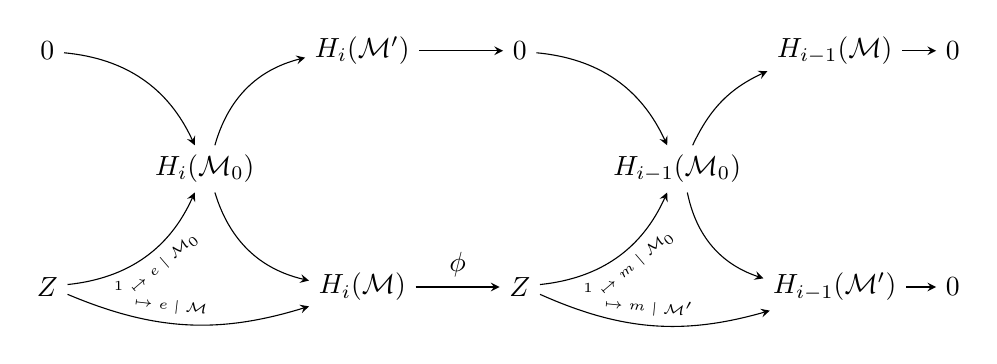
\begin{tikzpicture}
            \draw
                (-2, -1.5) node (B) {\(\mathbb{Z}\)}
                (0, 0) node (C) {\(H_i(\mathcal{M}_0)\)}
                (2, 1.5) node (D) {\(H_i(\mathcal{M}^{\prime})\)}
                (4, 1.5) node (E) {\(0\)}
                (-2, 1.5) node (G) {\(0\)}
                (2, -1.5) node (H) {\(H_i(\mathcal{M})\)}
                (4, -1.5) node (I) {\(\mathbb{Z}\)}
                (6, 0) node (J) {\(H_{i-1}(\mathcal{M}_0)\)}
                (8, 1.5) node (K) {\(H_{i-1}(\mathcal{M})\)}
                (8, -1.5) node (L) {\(H_{i-1}(\mathcal{M}^{\prime})\)}
                (9.5, -1.5) node (M) {\(0\)}
                (9.5, 1.5) node (N) {\(0\)}
                
                (B) edge [bend right = 30, -stealth] node [below = 0.17, pos = 0.31] {\tiny\(1\)} node [sloped, below, pos = 0.57] {\tiny\(\mapsto\eqcl{e\mathrel{|}\mathcal{M}_0}\)} (C)
                (B) edge [bend right = 20, -stealth] node [sloped, above, pos = 0.42] {\tiny\(\mapsto\eqcl{e\mathrel{|}\mathcal{M}}\)} (H)
                (C) edge [bend left = 30, -stealth] (D)
                (D) edge [-stealth] (E)
                (E) edge [bend left = 30, -stealth] (J)
                (J) edge [bend right = 30, -stealth] (L)
                (L) edge [-stealth] (M)

                (G) edge [bend left = 30, -stealth] (C)
                (C) edge [bend right = 30, -stealth] (H)
                (H) edge [-stealth] node [above] {\(\phi\)} (I)
                (I) edge [bend right = 30, -stealth] node [below = 0.17, pos = 0.29] {\tiny\(1\)} node [sloped, below, pos = 0.57] {\tiny\(\mapsto\eqcl{m\mathrel{|}\mathcal{M}_0}\)}  (J)
                (I) edge [bend right = 20, -stealth] node [sloped, above, pos = 0.47] {\tiny\(\mapsto\eqcl{m\mathrel{|}\mathcal{M}^{\prime}}\)}  (L)
                (J) edge [bend left = 20, -stealth] (K)
                (K) edge [-stealth] (N)
                ;
        \end{tikzpicture}
    \end{center}
    Wegen der Primitivit\"at ist \(\phi\colon H_i(\mathcal{M})\to\mathbb{Z},\,x\mapsto x\cdot\eqcl{\mathcal{S}\mathrel{|}\mathcal{M}}\) ein Epimorphismus, also folgt
    \[H_{i-1}(\mathcal{M}^{\prime})\cong H_{i-1}(\mathcal{M}_0)\cong H_{i-1}(\mathcal{M})\,.\]
    Weiter gilt
    \[H_i(\mathcal{M}^{\prime})\cong H_i(\mathcal{M}_0)/\langle\eqcl{e\mathrel{|}\mathcal{M}_0}\rangle\cong\ker\phi/\langle\eqcl{e\mathrel{|}\mathcal{M}}\rangle\,.\]
    Wegen \(\ker\phi\subseteq H_i(\mathcal{M})\) wird \(\eqcl{\mathcal{S}\mathrel{|}\mathcal{M}}\) eliminiert, wo\-m\"og\-lich mehr.
\end{proof}